\documentclass[12pt,a4paper]{article}
\usepackage[utf8]{inputenc}
% ===== 基本设置 =====
\usepackage[utf8]{inputenc}
\usepackage{graphicx}
\usepackage{longtable}
\usepackage{booktabs}
\usepackage{hyperref}
\usepackage{geometry}
\geometry{margin=1in}
\usepackage{setspace}
\setstretch{1.2}
\usepackage{caption}
\usepackage{amsmath}
\usepackage{textgreek}
\usepackage{newunicodechar}
\newunicodechar{▶}{\ding{220}} % or replace with a suitable symbol

% ===== 文档信息 =====
\title{\textbf{SECM V0.5 ALPHA Simulator User Manual}}
\author{Xiaofei Feng \\ Independent Researcher}
\date{\today}

\begin{document}

% ===== 封面 =====
\maketitle
\thispagestyle{empty}
\newpage

% ===== 目录 =====
\tableofcontents
\newpage

% ===== 第一章 Introduction =====
\section{Introduction}

The Societal Evolution Computational Model (SECM) V0.5 ALPHA is a 
time-agnostic computational framework designed to analyze the co-evolution 
of three core societal dimensions:

\begin{itemize}
    \item \textbf{Productive Capacity (X)} – A composite indicator 
    reflecting national economic productivity, including primary energy 
    consumption, animal power, and the equivalent productivity of human labor.
    
    \item \textbf{Societal Stress (Y)} – An aggregated measure of 
    internal social tensions and systemic costs.
    
    \item \textbf{Net Tension Drivers (Z)} – A dimensionless index that 
    determines the direction of societal stress movement, influenced by 
    technological dividends, inequality, and social complexity.
\end{itemize}

Unlike conventional forecasting models, SECM does not attempt to predict specific events or dates.  
Instead, it focuses on identifying \textbf{structural relationships} and \textbf{ratio dynamics} 
that govern societal evolution. The model's theoretical foundation draws from 
historical materialism, capturing the ``wave-like'' and ``spiral'' patterns 
observed in human societal development.

\subsection{Core Concepts}
\begin{enumerate}
    \item Growth in productive capacity (\(X\)) often leads to 
    increases in societal stress (\(Y\)), unless offset by sufficient 
    technological dividends or structural reforms.
    
    \item Societal carrying capacity (\(Y_{\text{limit}}\)) represents 
    the maximum sustainable level of societal stress before a systemic 
    breakdown occurs.
    
    \item When \(Y\) exceeds \(Y_{\text{limit}}\), an \textit{overshoot} 
    occurs, frequently followed by a crisis or contraction.
    
    \item The Z-axis (\(Z\)) acts as a predictive indicator: 
    rising \(Z\) often precedes crises, while declining \(Z\) can 
    indicate approaching relief phases.
    
    \item Declines in \(X\) cause \(Y_{\text{limit}}\) to drop faster 
    than \(Y\), increasing societal fragility.
\end{enumerate}

\subsection{Purpose of This Manual}
This user manual provides step-by-step guidance for installing, configuring, 
and operating the SECM V0.5 ALPHA Simulator. It is designed for both 
\textbf{non-technical users} and \textbf{researchers} who wish to 
reproduce, explore, and analyze historical or hypothetical societal 
evolution scenarios.

\noindent
Through detailed explanations, annotated interface descriptions, and worked examples, 
readers will be able to:
\begin{itemize}
    \item Prepare and format input datasets.
    \item Run simulations using national presets or custom parameters.
    \item Interpret outputs, including time-series plots and 
    early-warning indicators.
    \item Export and document results for further analysis.
\end{itemize}

\newpage
% ===== 第二章 =====
\section{System Requirements \& Installation}

\subsection{System Requirements}
The SECM V0.5 ALPHA Simulator is a standalone Windows application.  
No additional development environment is required.

\begin{itemize}
    \item \textbf{Operating System:} Windows 10 or later (64-bit)
    \item \textbf{Runtime Environment:} Microsoft .NET 8 Desktop Runtime
    \item \textbf{Processor:} Dual-core CPU (Intel i3 / AMD Ryzen 3 or higher recommended)
    \item \textbf{Memory:} 4 GB RAM (8 GB or more recommended for large datasets)
    \item \textbf{Storage:} 200 MB free disk space
    \item \textbf{Display:} 1366x768 resolution or higher
\end{itemize}

\noindent
The .NET 8 Desktop Runtime can be downloaded from the official Microsoft website:  
\url{https://dotnet.microsoft.com/en-us/download/dotnet/8.0}

\subsection{File Structure}
The simulator package contains the following files after extraction:
\begin{itemize}
    \item \texttt{SECM\_Simulator.exe} – Main executable file.
    \item \texttt{Presets/} – Folder containing JSON parameter presets for specific countries.
    \item \texttt{SampleData/} – Example datasets in CSV/Excel format.
    \item \texttt{Docs/} – Documentation files, including this manual.
    \item \texttt{Logs/} – Automatically generated logs during simulation runs.
\end{itemize}

\subsection{Installation Steps}
\begin{enumerate}
    \item Download the simulator package (\texttt{.zip}) from the official repository.
    \item Extract the contents to a dedicated folder on your computer.
    \item Install the Microsoft .NET 8 Desktop Runtime if not already installed.
    \item Double-click \texttt{SECM\_Simulator.exe} to launch the application.
    \item On first launch, verify that the interface loads correctly and that no runtime errors occur.
\end{enumerate}

\subsection{First-Time Setup Tips}
\begin{itemize}
    \item Keep all files within the extracted folder to ensure the simulator can access presets and sample data.
    \item If using custom datasets, store them in a separate folder and avoid overwriting the sample files.
    \item For high-resolution displays, enable display scaling in Windows settings for better readability.
\end{itemize}

\newpage
% ===== 第三章 =====
\section{User Interface Overview}

The SECM V0.5 ALPHA Simulator interface consists of four main areas:

\begin{enumerate}
    \item \textbf{Control Buttons Area} – Used to run, reset, import/export data, and manage presets.
    \item \textbf{General Input Data Area} – Contains all annual socio-economic input fields.
    \item \textbf{Parameter Input Area} – Allows adjustment of model coefficients and sensitivity factors.
    \item \textbf{Output and Log Area} – Displays simulation progress, numerical outputs, and visual charts.
\end{enumerate}

\subsection{Main Window Layout}
\begin{center}
    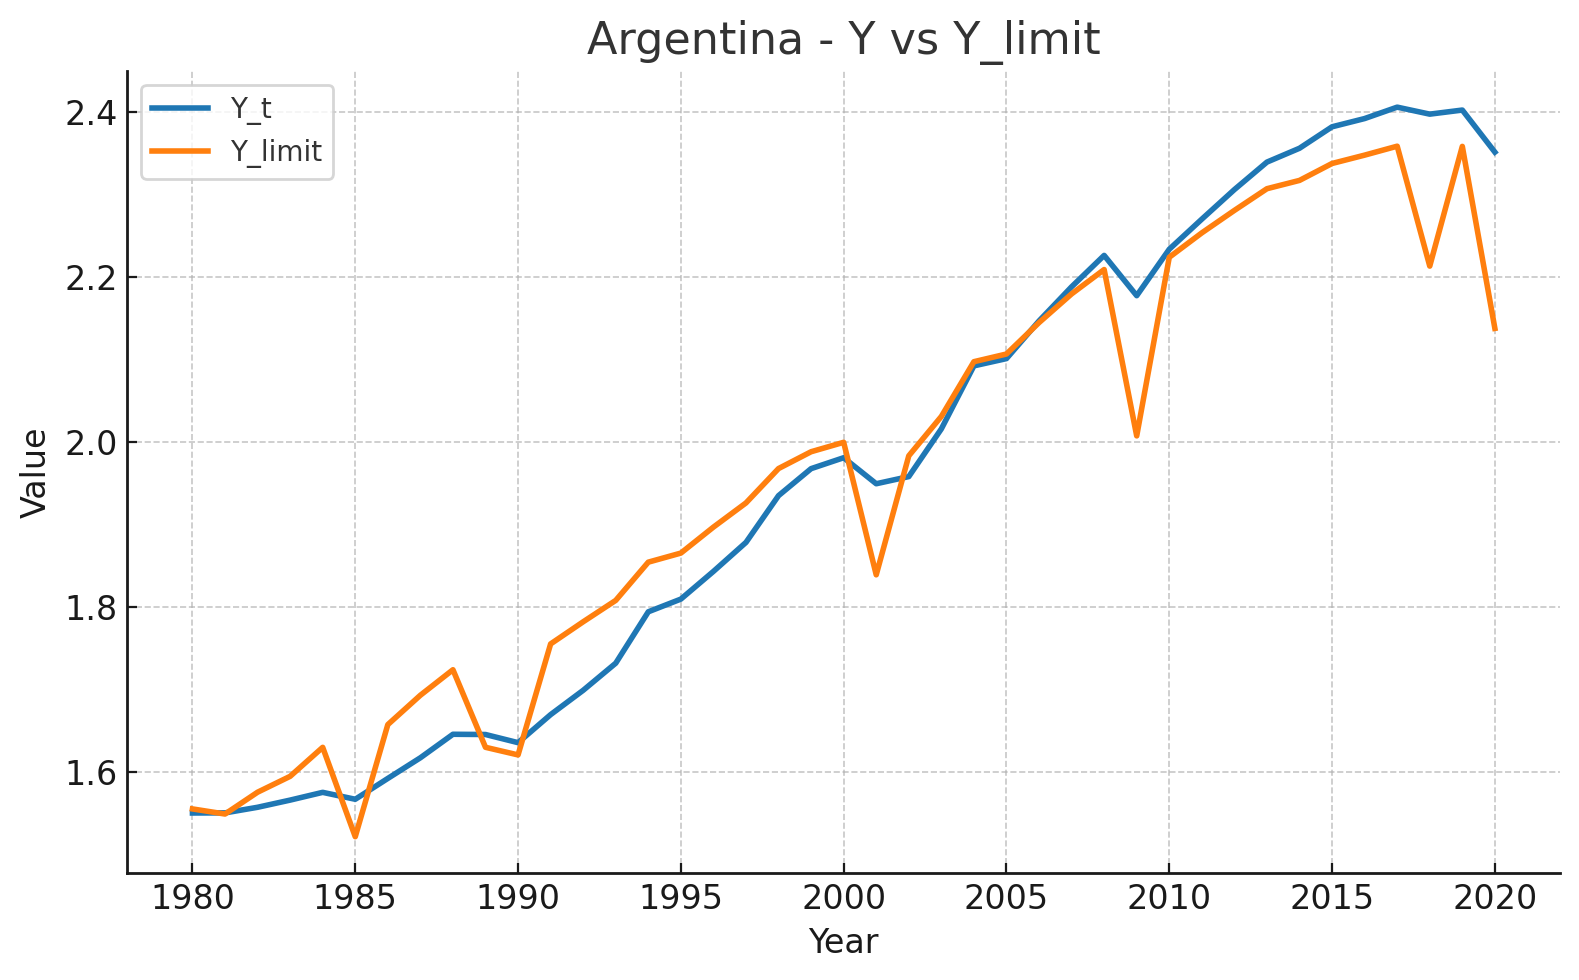
\includegraphics[width=0.85\textwidth]{1.png}
    \captionof{figure}{SECM V0.5 ALPHA Simulator Main Interface}
\end{center}

% ---- 按钮控件表 ----
\subsection{Control Buttons}
\begin{longtable}{p{3cm} p{4cm} p{8cm}}
\toprule
\textbf{Control Name} & \textbf{UI Label} & \textbf{Function} \\
\midrule
btnRun & \texttt{Run Simulation} & Execute the simulation with current input and parameter values. \\
btnClear & \texttt{Clear Inputs} & Clear all input fields. \\
btnReset & \texttt{Reset Defaults} & Restore default presets or load first row from Excel. \\
btnExportCSV & \texttt{Export CSV} & Export simulation history to a CSV file. \\
btnPlotChart & \texttt{View Chart} & Generate visual charts from simulation data. \\
btnClearLog & \texttt{Clear Log} & Clear the log output window. \\
btnExit & \texttt{Exit} & Exit the simulator. \\
btnLoadNation & \texttt{Load Country Preset} & Load national parameter preset (JSON). \\
btnSaveNation & \texttt{Save as Preset} & Save current parameters as a JSON preset. \\
btnImportExcel & \texttt{Import Excel} & Load input data from an Excel file. \\
btnExportExcel & \texttt{Export Excel} & Export simulation results to Excel. \\
\bottomrule
\end{longtable}


% ---- 现实输入项表 ----
\subsection{General Input Data Fields}
\begin{longtable}{p{4cm} p{4cm} p{7cm}}
\toprule
\textbf{UI Label} & \textbf{Textbox Name} & \textbf{Description} \\
\midrule
Year & \texttt{txtYear} & Simulation year for the current input row. \\
Population & \texttt{txtPopulation} & Total population (persons). \\
Population (Last Year) & \texttt{txtPopulationLast} & Population in the previous year. \\
Primary Energy (kWh) & \texttt{txtPrimaryEnergy} & Annual primary energy consumption in kWh. \\
Primary Energy (Last Year) & \texttt{txtPrimaryEnergyLast} & Primary energy consumption in previous year. \\
Animal Power (kWh) & \texttt{txtAnimalPower} & Estimated annual mechanical energy from animal labor. \\
Animal Power (Last Year) & \texttt{txtAnimalPowerLast} & Animal power in the previous year. \\
Patent Count & \texttt{txtPatentCount} & Number of patents filed in the current year. \\
Patent Count (Last Year) & \texttt{txtPatentLast} & Number of patents filed in the previous year. \\
Bonus θ (Theta) & \texttt{txtBonusTheta} & Coefficient for technology bonus calculation. \\
Bonus P & \texttt{txtBonusP} & Exponent in productivity growth component for bonus calculation. \\
Education Rate (\%) & \texttt{txtEduRate} & Share of population with higher education. \\
STEM Workforce Share (\%) & \texttt{txtSTEMShare} & Share of labor force in STEM fields. \\
TFP Growth (\%) & \texttt{txtTFPGrowth} & Total Factor Productivity growth rate. \\
Gini Coefficient & \texttt{txtGini} & Gini index for inequality (0–1). \\
Trust Index & \texttt{txtTrust} & Social trust index (0–1). \\
Savings Rate (\%) & \texttt{txtSavingsRate} & Household savings rate. \\
Debt Ratio (\%) & \texttt{txtDebtRate} & Household debt as \% of GDP. \\
Unemployment Rate (\%) & \texttt{txtUnemploymentRate} & Unemployment rate. \\
Military Expenditure (\% of GDP) & \texttt{txtMilitaryRatio} & Military spending as \% of GDP. \\
Market Cap / GDP Ratio & \texttt{txtMCapGDP} & Stock market capitalization / GDP. \\
Arable Land per Capita (ha/person) & \texttt{txtArableLandCapita} & Arable land per person. \\
Logistics Performance Index (0–5) & \texttt{txtLPI} & World Bank LPI score. \\
Healthcare Coverage (\%) & \texttt{txtHealthcareCoverage} & Population with healthcare access. \\
Pension Coverage (\%) & \texttt{txtPensionCoverage} & Population with pension access. \\
Free Education Coverage (\%) & \texttt{txtFreeEduCoverage} & Population with free education access. \\
Unemployment Insurance Coverage (\%) & \texttt{txtUnempInsCoverage} & Population with unemployment insurance. \\
Social Security Index (0–1) & \texttt{txtSocialSecIndex} & Composite index of social safety net. \\
Z Shock & \texttt{txtZShock} & External social destabilization shock. \\
Omega Shock & \texttt{txtOmegaShock} & External structural resilience shock. \\
Murder Rate (\%) & \texttt{txtMurderRate} & Annual homicide rate. \\
Poverty Rate (\%) & \texttt{txtPovertyRate} & Population below poverty line. \\
Gamma S & \texttt{txtGammaS} & Sensitivity coefficient for Z from social complexity. \\
Gamma X & \texttt{txtGammaX} & Sensitivity coefficient for Z from technology bonus. \\
Drift & \texttt{txtDrift} & Long-term Z-axis drift. \\
Zc Weight (w\_Zc) & \texttt{txtZcWeight} & Weight multiplier for Zc. \\
YBase A0 & \texttt{txtYBaseA0} & Coefficient A0 for Y\_base. \\
YBase B1 & \texttt{txtYBaseB1} & Coefficient B1 for Y\_base. \\
YBase A1 & \texttt{txtYBaseA1} & Coefficient A1 for Y\_base. \\
Mu Y0 & \texttt{txtMuY0} & Baseline Y adjustment parameter. \\
Land Cap Limit Coefficient & \texttt{txtLandCapLimitCoef} & Coefficient for land capacity limit. \\
K Limit & \texttt{txtKLimit} & Scaling factor for Y\_limit. \\
K Y & \texttt{txtKY} & Coefficient linking X to Y production. \\
S Decay Rate & \texttt{txtSDecayRate} & Decay rate for crisis pool S\_t. \\
K S & \texttt{txtKS} & Scaling factor for S\_t accumulation. \\
S0 (Initial Crisis Pool) & \texttt{txtS0} & Initial S\_t value. \\
Initial Y (First Year) & \texttt{txtYFirst} & Initial Y\_t value for first year. \\
\bottomrule
\end{longtable}

\newpage
% ===== 第四章 =====
\section{Data Preparation}

Before running simulations, the SECM V0.5 ALPHA Simulator requires structured input datasets.  
This chapter explains where to obtain the data, how to format it, and how to handle missing values.

\subsection{Data Sources}
The simulator can work with either:
\begin{itemize}
    \item Official historical datasets (recommended for backtesting).
    \item Custom datasets created by the user for hypothetical or counterfactual scenarios.
\end{itemize}

For historical testing, official data sources are available via the project’s GitHub repository:

\begin{itemize}
    \item \textbf{Main dataset (1980–2020)}: \url{https://github.com/Strangethought2025/SECM-Project/tree/main/Data/DATAsource/1980_2020%20Source}
    \item \textbf{Extreme test datasets}: \url{https://github.com/Strangethought2025/SECM-Project/tree/main/Data/DATAsource/ExtremeTest%20Source}
    \item \textbf{Bibliographic references}: \url{https://github.com/Strangethought2025/SECM-Project/blob/main/Data/DATAsource/1980_2020%20Source/Citation.xlsx}
\end{itemize}

\noindent
These datasets include raw values as well as \textbf{LOCF-processed} (Last Observation Carried Forward) values for missing entries.

\subsection{File Format Requirements}
\begin{itemize}
    \item Accepted formats: \texttt{.xlsx}, \texttt{.csv}
    \item Each row represents a year of data.
    \item Columns must correspond to the simulator’s \textbf{General Input Data Fields} (see Chapter 3).
    \item The first row should contain headers matching the simulator’s expected field names.
    \item All numerical values should be in standard decimal notation (dot as decimal separator).
\end{itemize}

\noindent
\textbf{Example header row:}
\begin{verbatim}
Year,Population,PopulationLast,PrimaryEnergy,PrimaryEnergyLast,
AnimalPower,AnimalPowerLast,PatentCount,PatentLast,BonusTheta,BonusP,
EduRate,STEMShare,TFPGrowth,Gini,Trust,SavingsRate,DebtRate,
UnemploymentRate,MilitaryRatio,MCapGDP,ArableLandCapita,LPI,
HealthcareCoverage,PensionCoverage,FreeEduCoverage,UnempInsCoverage,
SocialSecIndex,ZShock,OmegaShock,MurderRate,PovertyRate,
GammaS,GammaX,Drift,ZcWeight,YBaseA0,YBaseB1,YBaseA1,MuY0,
LandCapLimitCoef,KLimit,KY,SDecayRate,KS,S0,YFirst
\end{verbatim}

\subsection{Handling Missing Data (LOCF Method)}
The simulator is not tolerant of blank cells in the input dataset.  
If official datasets have missing values, the \textbf{LOCF method} is used:
\begin{itemize}
    \item If a year’s value is missing, use the last available value from a previous year.
    \item LOCF maintains trend continuity and avoids artificial spikes caused by interpolation.
\end{itemize}

\subsection{Importing Data into the Simulator}
\begin{enumerate}
    \item Click \texttt{Import Excel} or \texttt{Import CSV} in the \textbf{Control Buttons Area}.
    \item Browse to your dataset file and open it.
    \item Verify that all fields are correctly populated in the \textbf{General Input Data Area}.
    \item If using a preset dataset from the GitHub repository, no further adjustments are required.
\end{enumerate}

\subsection{Using Preset Country Parameters}
Alongside datasets, the simulator uses parameter presets stored as \texttt{.json} files in the \texttt{Presets/} directory.
\begin{itemize}
    \item Load a preset via \texttt{Load Country Preset} before importing the dataset.
    \item Presets contain fixed coefficients such as \(k_Y\), \(k_{\text{Limit}}\), and technology bonus parameters.
    \item You may edit presets in a text editor to create custom parameter sets.
\end{itemize}

\newpage
% ===== 第五章 =====
\section{Basic Operation}

This chapter provides a complete walk-through of running a simulation using the SECM V0.5 ALPHA Simulator.  
For illustration, we use the historical dataset for the \textbf{United States (1980–2020)}.

\subsection{Step 1 – Launch the Simulator}
\begin{enumerate}
    \item Double-click \texttt{SECM\_Simulator.exe} to open the program.
    \item The main interface will load, displaying the \textbf{Control Buttons Area}, \textbf{General Input Data Area}, \textbf{Parameter Input Area}, and \textbf{Log/Output Area}.
\end{enumerate}

\subsection{Step 2 – Load a Country Parameter Preset}
\begin{enumerate}
    \item Click \texttt{Load Country Preset}.
    \item Select the file \texttt{USA.json} from the \texttt{Presets/} folder.
    \item The \textbf{Parameter Input Area} will be populated with the recommended coefficients for the United States.
\end{enumerate}

\noindent
\textbf{Tip:} Always load the preset before importing data to ensure correct parameter alignment.

\subsection{Step 3 – Import the Dataset}
\begin{enumerate}
    \item Click \texttt{Import Excel}.
    \item Navigate to \texttt{SampleData/USA\_1980\_2020.xlsx}.
    \item Confirm that all fields in the \textbf{General Input Data Area} are correctly filled.
\end{enumerate}

\subsection{Step 4 – Verify Initial Y Value (\texttt{YFirst})}
\begin{enumerate}
    \item In the \textbf{Parameter Input Area}, check the \texttt{Initial Y (First Year)} field (\texttt{txtYFirst}).
    \item If using the official dataset, this value will be pre-set based on historical calibration.
    \item For custom datasets, set \texttt{YFirst} to a realistic starting societal stress level.
\end{enumerate}

\subsection{Step 5 – Run the Simulation}
\begin{enumerate}
    \item Click \texttt{Run Simulation}.
    \item The \textbf{Log/Output Area} will display year-by-year results as the model iterates.
    \item Progress indicators and key variables (X, Y, \(Y_{\text{limit}}\), Z) will update in real-time.
\end{enumerate}

\subsection{Step 6 – View Charts}
\begin{enumerate}
    \item Once the simulation completes, click \texttt{View Chart}.
    \item A visual plot of \(Y\) and \(Y_{\text{limit}}\) over time will be generated.
    \item Additional plots (e.g., \(Y\) vs. \(Z\)) can be exported for analysis.
\end{enumerate}

\begin{center}
    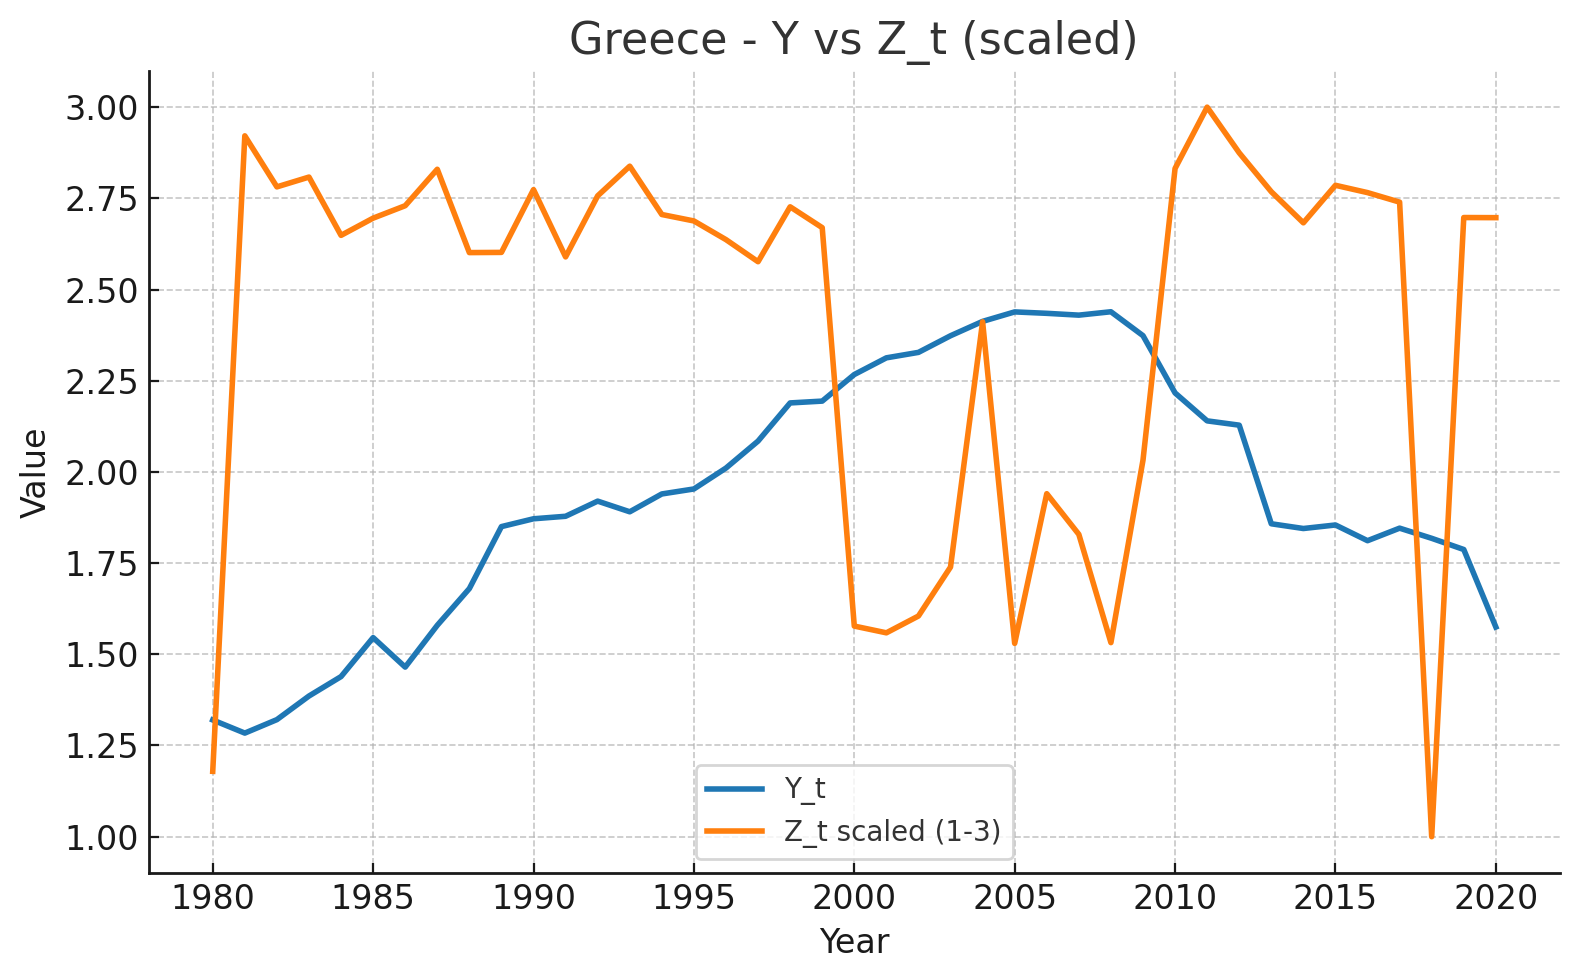
\includegraphics[width=0.85\textwidth]{2.png}
    \captionof{figure}{Example output chart: Y vs. Y\_limit for the Greece}
\end{center}

\subsection{Step 7 – Export Results}
\begin{enumerate}
    \item To export numeric results, click \texttt{Export CSV} or \texttt{Export Excel}.
    \item Choose a save location and filename.
    \item The exported file will contain yearly values for all calculated variables, allowing further analysis in Excel, R, or Python.
\end{enumerate}

\subsection{Step 8 – Reset or Exit}
\begin{itemize}
    \item Click \texttt{Reset Defaults} to clear results and prepare for another run.
    \item Click \texttt{Exit} to close the simulator.
\end{itemize}


\newpage
% ===== 第六章 =====
\section{Advanced Features}

Beyond basic simulation runs, the SECM V0.5 ALPHA Simulator provides several advanced capabilities for research and scenario testing.

\subsection{Parameter Adjustment}
The \textbf{Parameter Input Area} contains coefficients that influence the model’s behavior.  
Adjusting these values allows for:
\begin{itemize}
    \item Testing model sensitivity to specific societal factors.
    \item Simulating alternative policy or development paths.
    \item Calibrating the model to match new datasets or countries.
\end{itemize}

\noindent
Key parameters include:
\begin{itemize}
    \item \(k_Y\) – Links productive capacity \(X\) to societal stress \(Y\).
    \item \(k_{\text{Limit}}\) – Scales the societal carrying capacity \(Y_{\text{limit}}\).
    \item \(\theta\) (Bonus Theta) – Weight for technology bonus.
    \item \(P\) (Bonus P) – Exponent for productivity-driven bonus growth.
    \item \(\gamma_S\) and \(\gamma_X\) – Sensitivity coefficients for Z-axis response.
    \item \(S_0\) – Initial crisis pool value.
\end{itemize}

\subsection{Extreme Testing (Stress Tests)}
Extreme testing involves deliberately altering inputs to observe model stability and response patterns.
Two main approaches are:
\begin{enumerate}
    \item \textbf{Timeframe compression} – Shortening the dataset period to check whether the model preserves long-term trends.
    \item \textbf{Variable extremes} – Artificially increasing or decreasing a key input (e.g., \(Y\) or \(Y_{\text{limit}}\)) to test how the system responds.
\end{enumerate}

\noindent
\textbf{Example: Greece Y-limit Test}
\begin{itemize}
    \item Input: Historical dataset for Greece (1980–2020).
    \item Modification: Multiply \(Y_{\text{limit}}\) by 1.5 for all years.
    \item Observation: The \(Y\) curve shifts relative to \(Y_{\text{limit}}\) without destabilizing the long-term pattern, confirming model resilience.
\end{itemize}

\subsection{External Shock Variables}
The simulator includes two special input fields for simulating shocks:
\begin{itemize}
    \item \textbf{ZShock} – External social destabilization (e.g., political polarization).  
    Positive values increase societal stress; negative values represent positive events.
    \item \textbf{OmegaShock} – External structural resilience shock (e.g., natural disasters or infrastructure upgrades).  
    Positive values reduce carrying capacity; negative values improve resilience.
\end{itemize}

\noindent
\textbf{Usage:}
\begin{enumerate}
    \item Enter shock values directly in the input field for the year in question.
    \item Run the simulation to observe how the shock propagates through \(Y\), \(Y_{\text{limit}}\), and \(Z\).
\end{enumerate}

\subsection{Technology Bonus Analysis}
The technology bonus (\(X_{\text{bonus}}\)) reflects the combined effect of education, STEM workforce share, patent activity, and TFP growth:
\[
X_{\text{bonus},t} = \theta \cdot \text{STEM}_t \cdot \text{EduRate}_t \cdot (1 + \text{TFP}_t) \cdot \left( 1 + \frac{\text{PatentDensity}_t}{\text{PatentDensity}_{t-1}} \right) \cdot \left( 1 + \frac{X_t}{X_{t-1}} \right)^P
\]
where:
\[
\text{PatentDensity}_t = \frac{\text{PatentCount}_t}{\text{Population}_t / 10^6}
\]

\noindent
Increasing \(\theta\) or \(P\) amplifies the effect of technological progress on reducing societal stress.

\subsection{Stability Verification (Pearson Correlation Test)}
A stability check can be performed by running the model with different dataset lengths (e.g., 10-year vs. 40-year periods) and comparing the output curves using Pearson’s correlation coefficient:
\[
r = \frac{\sum (Y_t - \overline{Y})(\hat{Y}_t - \overline{\hat{Y}})}{\sqrt{\sum (Y_t - \overline{Y})^2 \cdot \sum (\hat{Y}_t - \overline{\hat{Y}})^2}}
\]
Values of \(r \approx 1.0\) indicate extremely high stability across different timescales.

\newpage
% ===== 第七章 =====
\section{Frequently Asked Questions (FAQ)}

This section addresses common issues users may encounter when using the SECM V0.5 ALPHA Simulator.

\subsection*{1. The program shows an error when importing data}
\textbf{Possible causes:}
\begin{itemize}
    \item The file format is unsupported (\texttt{.xls} instead of \texttt{.xlsx} or \texttt{.csv}).
    \item Column headers do not match the required field names.
    \item Missing values have not been filled using the LOCF method.
\end{itemize}
\textbf{Solutions:}
\begin{itemize}
    \item Save your Excel file as \texttt{.xlsx} or \texttt{.csv}.
    \item Ensure headers exactly match the expected names (see Chapter 3).
    \item Apply LOCF to fill missing values before import.
\end{itemize}

\subsection*{2. Output curves look unrealistic or flat}
\textbf{Possible causes:}
\begin{itemize}
    \item Incorrect parameter preset for the country.
    \item Initial Y value (\texttt{YFirst}) is set too high or too low.
    \item Extreme or unrealistic input values.
\end{itemize}
\textbf{Solutions:}
\begin{itemize}
    \item Load the correct country preset before running the simulation.
    \item Adjust \texttt{YFirst} to a reasonable starting value.
    \item Review input dataset for errors or unrealistic values.
\end{itemize}

\subsection*{3. Changing parameters seems to have no effect}
\textbf{Possible causes:}
\begin{itemize}
    \item The parameter being changed has minimal impact for the given dataset.
    \item Changes are too small to produce visible effects in short runs.
\end{itemize}
\textbf{Solutions:}
\begin{itemize}
    \item Try larger adjustments to parameters (e.g., change \(\theta\) from 1.0 to 1.5).
    \item Extend the simulation period to observe cumulative effects.
\end{itemize}

\subsection*{4. I get blank charts after running the simulation}
\textbf{Possible causes:}
\begin{itemize}
    \item The simulation did not run to completion.
    \item No output data was generated due to missing or invalid inputs.
\end{itemize}
\textbf{Solutions:}
\begin{itemize}
    \item Ensure all required fields are filled before starting the simulation.
    \item Check the log window for errors during execution.
\end{itemize}

\subsection*{5. How do I test the impact of a major event?}
\textbf{Answer:}
Use the \texttt{ZShock} or \texttt{OmegaShock} fields for the year of the event:
\begin{itemize}
    \item Positive \texttt{ZShock} simulates increased societal stress (e.g., political crisis).
    \item Negative \texttt{ZShock} simulates a positive development (e.g., major peace agreement).
    \item Positive \texttt{OmegaShock} reduces carrying capacity (e.g., natural disaster).
    \item Negative \texttt{OmegaShock} increases resilience (e.g., infrastructure upgrade).
\end{itemize}

\subsection*{6. Where can I find sample datasets?}
\textbf{Answer:}
Sample datasets are included in the \texttt{SampleData/} folder and in the project’s GitHub repository.  
They cover 1980–2020 data for multiple countries, including the United States, Japan, Greece, and Argentina.

\newpage
% ===== 第八章 =====
\section{Appendix}

\subsection{A. Control Buttons Reference}
\begin{longtable}{p{3cm} p{4cm} p{8cm}}
\toprule
\textbf{Control Name} & \textbf{UI Label} & \textbf{Function} \\
\midrule
btnRun & \texttt{Run Simulation} & Execute simulation. \\
btnClear & \texttt{Clear Inputs} & Clear all input fields. \\
btnReset & \texttt{Reset Defaults} & Restore defaults or load first Excel row. \\
btnExportCSV & \texttt{Export CSV} & Export results as CSV. \\
btnPlotChart & \texttt{View Chart} & Generate simulation charts. \\
btnClearLog & \texttt{Clear Log} & Clear log output. \\
btnExit & \texttt{Exit} & Close the simulator. \\
btnLoadNation & \texttt{Load Country Preset} & Load parameter preset (JSON). \\
btnSaveNation & \texttt{Save as Preset} & Save parameters to JSON. \\
btnImportExcel & \texttt{Import Excel} & Import data from Excel file. \\
btnExportExcel & \texttt{Export Excel} & Export results to Excel file. \\
\bottomrule
\end{longtable}


\subsection{B. Input \& Parameter Field Mapping}
\begin{longtable}{p{4cm} p{4cm} p{7cm}}
\toprule
\textbf{UI Label} & \textbf{Textbox Name} & \textbf{Variable Purpose} \\
\midrule
Population & \texttt{txtPopulation} & Total population. \\
Primary Energy (kWh) & \texttt{txtPrimaryEnergy} & Annual primary energy consumption. \\
Animal Power (kWh) & \texttt{txtAnimalPower} & Annual animal labor energy. \\
Patent Count & \texttt{txtPatentCount} & Patents filed in current year. \\
Education Rate (\%) & \texttt{txtEduRate} & Higher education attainment. \\
STEM Workforce Share (\%) & \texttt{txtSTEMShare} & STEM sector employment share. \\
TFP Growth (\%) & \texttt{txtTFPGrowth} & Total Factor Productivity growth. \\
Gini Coefficient & \texttt{txtGini} & Inequality index. \\
Trust Index & \texttt{txtTrust} & Social trust level. \\
Savings Rate (\%) & \texttt{txtSavingsRate} & Household savings share. \\
Debt Ratio (\%) & \texttt{txtDebtRate} & Household debt share of GDP. \\
Unemployment Rate (\%) & \texttt{txtUnemploymentRate} & Jobless population share. \\
Military Expenditure (\% of GDP) & \texttt{txtMilitaryRatio} & Defense spending ratio. \\
Market Cap / GDP Ratio & \texttt{txtMCapGDP} & Stock market size relative to GDP. \\
Arable Land per Capita & \texttt{txtArableLandCapita} & Agricultural land per person. \\
LPI (0–5) & \texttt{txtLPI} & Logistics Performance Index. \\
Healthcare Coverage (\%) & \texttt{txtHealthcareCoverage} & Health service access rate. \\
Pension Coverage (\%) & \texttt{txtPensionCoverage} & Pension benefit coverage. \\
Free Education Coverage (\%) & \texttt{txtFreeEduCoverage} & Public education access. \\
Unemployment Insurance Coverage (\%) & \texttt{txtUnempInsCoverage} & Welfare coverage for unemployed. \\
Social Security Index (0–1) & \texttt{txtSocialSecIndex} & Composite welfare index. \\
ZShock & \texttt{txtZShock} & External societal stress shock. \\
OmegaShock & \texttt{txtOmegaShock} & External resilience shock. \\
Murder Rate (\%) & \texttt{txtMurderRate} & Homicide rate. \\
Poverty Rate (\%) & \texttt{txtPovertyRate} & Poverty share. \\
Gamma S & \texttt{txtGammaS} & Z sensitivity to social complexity. \\
Gamma X & \texttt{txtGammaX} & Z sensitivity to tech bonus. \\
\bottomrule
\end{longtable}

\subsection{C. Key Variables Explained (Simplified)}
\begin{itemize}
    \item \(X\) – Productive capacity, derived from energy, labor, and technology.
    \item \(Y\) – Societal stress level.
    \item \(Y_{\text{limit}}\) – Maximum sustainable \(Y\) before systemic breakdown.
    \item \(Z\) – Directional driver of \(Y\), integrating tech bonus, inequality, and complexity.
    \item \(X_{\text{bonus}}\) – Technological dividend improving system resilience.
    \item \(S_t\) – Crisis pool, accumulates when \(Y > Y_{\text{limit}}\).
\end{itemize}

\subsection{D. Data Sources and References}
\begin{itemize}
    \item World Bank – \textit{World Development Indicators}.
    \item United Nations – \textit{Population and Demographic Statistics}.
    \item International Energy Agency – \textit{Energy Balances}.
    \item OECD – \textit{STEM workforce and education statistics}.
    \item Project GitHub Repository: \url{https://github.com/Strangethought2025/SECM-Project}
\end{itemize}

\newpage

% ===== 结束 =====
\end{document}
